\section{Experiments and Results}

\subsection{Hardware Description}
% We used an Intel Xeon Sapphire Rapids CPU-equipped workstation running on 2.00GHz with 925 GB of memory and an Nvidia A100-SXM4-80GB GPU card with 80 GB of VRAM, 108 SMs, and 6912 CUDA cores.

The experiments were conducted on a high-performance computing node equipped with an Intel Xeon Gold 6548Y+ processor (5th Gen), providing 24 physical cores with a base frequency of 2.50 GHz (up to 4.10 GHz Turbo) and a 1.4 GiB L3 cache. The system features 1.5 TB of DDR5 RAM. Hardware acceleration was provided by an NVIDIA H100 NVL (94GB) GPU.

\subsection{Time Measurement Process and Correctness Checking}
Timing measurements were performed by invoking the algorithm as a library. The total execution time was measured from immediately before the function call to immediately after its completion, thereby accounting for all host–device data transfer overhead.

To assess both the performance and correctness of the proposed CUDA C++ GPU-based region extraction algorithms, we conducted a comprehensive comparison against a reference CPU implementation based on BGL, CGAL, and also our own C++ implementation of the algorithms.

When performing region extraction using the BGL library, it is necessary to first invoke a planarity testing function (boyer\_myrvold\_planarity\_test) to verify that the input graph is planar prior to extracting its faces. Although extracting the regions from the graph embedding, after calling the planarity test function, does not take much time, the planarity test itself introduces a considerable runtime overhead, which makes the BGL library not a practical approach when dealing with giant graphs whose planarity is already guaranteed. Therefore, in the Results section, we report only the time required for region extraction after validating the graphs, and only for the smallest graph instances, as including the planarity testing time would not provide a meaningful or practical performance comparison.

In contrast, the CGAL library does not require an explicit external call to a dedicated planarity testing function. Instead, it is designed with robustness and generality in mind, operating without the assumption that the input graph is already connected and planar. While the overall runtime of CGAL is reported, a direct comparison with the GPU-based implementation is not appropriate due to fundamental differences in design objectives and computational models.

Finally, we implemented the Wedge-based and the HE-based algorithms in standard C++ for execution on the CPU. All these implementations serve as a baseline for both correctness verification and runtime analysis, leveraging the prior knowledge that all experimental input graphs are valid connected planar graphs and therefore do not require explicit planarity testing.

% Region extraction in the BGL library works as follows: (boyer\_myrvold\_planarity\_test) function tests if the input graph can be drawn in a plane without edge crossings, and if it is planar, it creates a valid planar embedding.  Although extracting the regions from the graph embedding doesn't take much time, the function (boyer\_myrvold\_planarity\_test) takes a long time to test graph planarity, and it is a mandatory step while using BGL, which makes the BGL library not a practical approach when dealing with giant graphs that we are confident of their planarity. In the results section, we included only the time of extracting the regions from the graph embeddings, and only for the smallest graphs, because checking graph planarity takes much time, and it was not practical to include this time.

% CGAL's region extraction functions primarily accept geometric primitives—points, segments, polygons, or planar curves—as input, which define region boundaries through their spatial arrangement and intersections. The library processes these inputs by first constructing a planar arrangement, automatically computing all intersection points between input elements to decompose the plane into non-overlapping regions.

% Finally, we implemented the original algorithm~\cite{JIANG1993553} in normal C++ code that runs on CPU to use as a benchmark for correctness and time analysis to make use of our knowledge that the input graphs we used in the experiments are valid planar graphs, and there is no need to check their planarity.

\subsection{Data}
The evaluation was carried out on a suite of synthetic 2D mesh graphs designed to emulate the large-scale meshes commonly found in scientific and engineering applications. These test graphs varied in size and structure, with each graph representing a square grid of \(l \times l\) vertices, with \(l\) taking values from \(\{1001, 4001, 8001, 12001\}\), thereby covering a range from moderately sized to extremely large graphs.

Three distinct edge patterns were used to generate the test graphs, each designed to simulate different types of planar structures. The first pattern \((P_1)\) includes horizontal, vertical, and diagonal edges at most of the vertices, forming a dense mesh characterized by small triangular regions. The second pattern \((P_2)\) is sparser, resulting in a combination of small triangular regions and larger zigzag regions. The third pattern \((P_3)\) represents a hybrid configuration that blends features of the first two, producing regions of varying shapes and sizes, and offering a mid-density mesh.

Across all graph sizes and patterns, the CUDA C++ implementation consistently produced results identical to the CPU version, validating its correctness. Furthermore, it achieved substantial speedup, particularly for larger graphs, demonstrating the benefits of efficient parallelism in handling complex region extraction tasks.

Figures~\ref{fig:graph_pattern_1}, \ref{fig:graph_pattern_2}, and \ref{fig:graph_pattern_3} illustrate the structure of graph patterns \(P_1\), \(P_2\), and \(P_3\), respectively, using a small example with \(l = 7\), and Table~\ref{tab:graph_data} summarizes the corresponding graph statistics, including the number of vertices, edges, and regions extracted for each pattern.

\begin{figure}
    \centering
    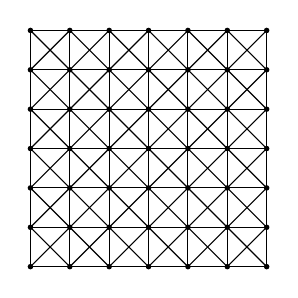
\begin{tikzpicture}[scale=0.5]
        % Define the size of the grid
\def\n{7}

\foreach \j in {0,...,\numexpr\n-1} {
    \foreach \i in {0,...,\numexpr\n-1} {
        \fill (\i,\j) circle[radius=2pt];  % black filled circle
    }
}

\foreach \j in {0,...,\numexpr\n-2} {
    \foreach \i in {0,...,\numexpr\n-1} {
        \draw (\i,\j) -- (\i,\j+1);
    }
}

\foreach \j in {0,...,\numexpr\n-1} {
    \foreach \i in {0,...,\numexpr\n-2} {
        \draw (\i,\j) -- (\i+1,\j);
    }
}

\foreach \j in {0,...,\numexpr\n-2} {
    \foreach \i in {0,...,\numexpr\n-2} {
        \pgfmathtruncatemacro{\sumval}{\i + \j}
        \ifthenelse{\isodd{\sumval}}
        {
            \draw (\i+1,\j) -- (\i,\j+1);
        }
        {
            \draw (\i,\j) -- (\i+1,\j+1);
        }
    }
}

    \end{tikzpicture}
    \caption{Pattern 1 of graphs for a grid of \(7 \times 7\) vertices}
    \label{fig:graph_pattern_1}
\end{figure}


\begin{figure}
    \centering
    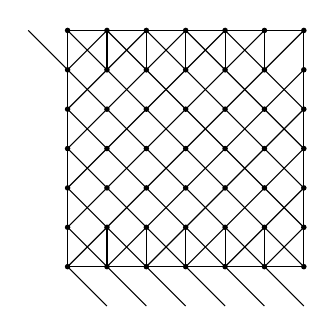
\begin{tikzpicture}[scale=0.5]
        % Define the size of the grid
\def\n{7}

\foreach \j in {0,...,\numexpr\n-1} {
    \foreach \i in {0,...,\numexpr\n-1} {
        \fill (\i,\j) circle[radius=2pt];  % black filled circle
    }
}

% Vertical lines on left and right edges
\foreach \j in {0,...,\numexpr\n-2} {
    \draw (0,\j) -- (0,\j+1);
    \draw (\numexpr\n-1,\j) -- (\numexpr\n-1,\j+1);
    
    \foreach \i in {0,...,\numexpr\n-2} {
        \ifthenelse{\isodd{\i}}{
            \draw (\i,\j) -- (\i+1,\j+1);
        }{
            \ifthenelse{\j > 0}{
                \draw (\i,\j) -- (\i+1,\j-1);
            }{}
        }
    }
}

% Horizontal lines on top and bottom edges
\foreach \i in {0,...,\numexpr\n-2} {
    \draw (\i,0) -- (\i+1,0);
    \draw (\i,\numexpr\n-1) -- (\i+1,\numexpr\n-1);
    
    \ifthenelse{\isodd{\i}=0}{
        \draw (\i-1,\numexpr\n-1) -- (\i,\numexpr\n-2);
    }{}
    
    \ifthenelse{\i > 0}{
        \ifthenelse{\isodd{\i}=0}{
            \draw (\i,\numexpr\n-2) -- (\i,\numexpr\n-1);
        }{
            \draw (\i,0) -- (\i,1);
        }
    }{}
}
    \end{tikzpicture}
    \caption{Pattern 2 of graphs for a grid of \(7 \times 7\) vertices}
    \label{fig:graph_pattern_2}
\end{figure}

\begin{figure}
    \centering
    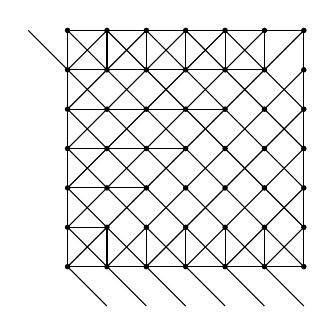
\begin{tikzpicture}[scale=0.5]
        % Define the size of the grid
\def\n{7}

\foreach \j in {0,...,\numexpr\n-1} {
    \foreach \i in {0,...,\numexpr\n-1} {
        \fill (\i,\j) circle[radius=2pt];  % black filled circle
    }
}

% Vertical lines on left and right edges
\foreach \j in {0,...,\numexpr\n-2} {
    \draw (0,\j) -- (0,\j+1);
    \draw (\numexpr\n-1,\j) -- (\numexpr\n-1,\j+1);
    
    \foreach \i in {0,...,\numexpr\n-2} {
        \ifthenelse{\isodd{\i}}{
            \draw (\i,\j) -- (\i+1,\j+1);
        }{
            \ifthenelse{\j > 0}{
                \draw (\i,\j) -- (\i+1,\j-1);
            }{}
        }
    }
}

% Horizontal lines on top and bottom edges
\foreach \i in {0,...,\numexpr\n-2} {
    \draw (\i,0) -- (\i+1,0);
    \draw (\i,\numexpr\n-1) -- (\i+1,\numexpr\n-1);
    
    \ifthenelse{\isodd{\i}=0}{
        \draw (\i-1,\numexpr\n-1) -- (\i,\numexpr\n-2);
    }{}
    
    \ifthenelse{\i > 0}{
        \ifthenelse{\isodd{\i}=0}{
            \draw (\i,\numexpr\n-2) -- (\i,\numexpr\n-1);
        }{
            \draw (\i,0) -- (\i,1);
        }
    }{}
}

% Outer loop: j from 1 to n-2
\foreach \j in {1,...,\numexpr\n-2} {
    % Inner loop: i from 0 to j-1 (since range(0, j))
    \foreach \i in {0,...,\numexpr\j-1} {
        % Draw line from (i, j) to (i+1, j)
        \draw (\i,\j) -- (\numexpr\i + 1,\j);
    }
}

% Draw grid lines
  % \draw[gray, dotted] (0, 0) grid (\numexpr\n-1, \numexpr\n-1);

    \end{tikzpicture}
    \caption{Pattern 3 of graphs for a grid of \(7 \times 7\) vertices}
    \label{fig:graph_pattern_3}
\end{figure}



\captionsetup[table]{skip=10pt}

\begin{table*}
\centering
\begin{tabularx}{\textwidth}{|X|X|X|X|X|X|}
% \begin{tabularx}{\textwidth}{|C|C|C|C|C|C|}
\hline
Graph ID & Pattern Grid Side Length \((l)\) & Pattern Type & Number of Vertices \((n)\) & Number of Edges \((m)\) & Number of Regions \\
\hline
\(g_1\) & 1,001 & \(P_1\) & 1,002,001 & 3,002,000 & 2,000,001 \\
\hline
\(g_2\) & 1,001 & \(P_2\) & 1,002,001 & 1,004,999 & 3,000 \\
\hline
\(g_3\) & 1,001 & \(P_3\) & 1,002,001 & 1,504,499 & 502,500 \\
\hline
\(g_4\) & 4,001 & \(P_1\) & 16,008,001 & 48,008,000 & 32,000,001 \\
\hline
\(g_5\) & 4,001 & \(P_2\) & 16,008,001 & 16,019,999 & 12,000 \\
\hline
\(g_6\) & 4,001 & \(P_3\) & 16,008,001 & 24,017,999 & 8,010,000 \\
\hline
\(g_7\) & 8,001 & \(P_1\) & 64,016,001 & 192,016,000 & 128,000,001 \\
\hline
\(g_8\) & 8,001 & \(P_2\) & 64,016,001 & 64,039,999 & 24,000 \\
\hline
\(g_9\) & 8,001 & \(P_3\) & 64,016,001 & 96,035,999 & 32,020,000 \\
\hline
\(g_{10}\) & 12,001 & \(P_1\) & 144,024,001 & 432,024,000 & 288,000,001 \\
\hline
\(g_{11}\) & 12,001 & \(P_2\) & 144,024,001 & 144,059,999 & 36,000 \\
\hline
\(g_{12}\) & 12,001 & \(P_3\) & 144,024,001 & 216,053,999 & 72,030,000 \\
\hline

\end{tabularx}
\caption{Graphs Data for Different Patterns and Sizes}
\label{tab:graph_data}
\end{table*}

\subsection{Results}

% For the different graphs mentioned in the table~\ref{tab:graph_data}, regions are extracted using the different CPU methods mentioned above (BGL, CGAL, and the original algorithm implemented on the CPU), and the time and the results are compared to the GPU implementation. The correctness is tested across the graphs, and the time speedup was calculated as the ratio between the GPU implementation time and the other CPU implementations time. As mentioned before, the time is calculated for the group of the graph with the smallest \(l\) where \(l = 1001\) for the BGL implementation. You can find the results in table~\ref{tab:results}. You can see from the table that the fastest CPU implementation is for our own C++ code, because it executes only the algorithm and doesn't do any planarity checks, and this is useful in our case, and as a result, we will focus on the comparison between it and the CUDA implementation. Figure~\ref{fig:speedup} illustrates the speedup between our CPU and the GPU implementations of the algorithm, where you can see that the speedup is increasing for larger graphs till it reaches $33\times$ for the largest graphs with an average speedup 50x. The resulting speedup values show the importance of using the GPU implementation.

For the graph instances listed in Table~\ref{tab:graph_data}, region extraction was performed using the four CPU-based approaches described above: BGL, CGAL libraries, and our own C++ implementations of the Wedge-based and the HE-based algorithms, and 2 GPU-based approaches, the Wedge-based and the HE-based. Correctness was verified across all graph instances, and the speedup of each implementation was computed as the ratio of the execution time to the HE-based GPU execution time, as the fastest run time results were for the HE-based algorithm either on the CPU or on the GPU for most of the test cases. It is noted that the GPU-accelerated HE-based algorithm is slightly faster than the GPU-accelerated Wedge-based algorithm. 

As mentioned previously, for the BGL implementation, timing measurements were limited to the smallest graph group ($l = 1001$), due to the overhead associated with planarity testing. The detailed results are presented in Table~\ref{tab:results}. Among the CPU approaches, our HE-based C++ implementation achieved better performance than the libraries, as it executes only the core algorithm without performing planarity checks, and better than the Wedge-based implementation, which was expected because it depends on the twin edges to find the next edges, and it does not need to do binary search. Comparing the two parallel approaches shows that the Half-Edge implementation consistently outperforms the Wedge-based framework. This advantage arises because the Half-Edge data structure tracks connectivity natively, avoiding the secondary wedge-sorting step required by the wedge algorithm, with the latter typically being up to 13\% slower across test cases. Consequently, the primary comparison focuses on this CPU implementation and the CUDA-based GPU implementation for the HE-based algorithm which are the fastest CPU and GPU implementations.

Figure~\ref{fig:speedup} illustrates the resulting speedup, demonstrating a clear increase in performance gains as the graph size grows. The speedup reaches up to $33\times$ for the largest graph instances, with an average speedup of $23.7\times$. These results highlight the significant performance benefits of the GPU-based implementation. Pattern 1 exhibits lower speedup due to significant load imbalance caused by its non-uniform region distribution. The algorithm's parallel efficiency depends on the maximum region size; since Pattern 1 is dominated by one massive exterior region (with size $4(l+1)$) alongside many small triangular regions, GPU threads must wait for the largest region to process. High speedup is more readily achieved in patterns where region sizes are homogeneous, ensuring a balanced workload.

% The reason why the speedup of pattern 1 is much less than the other patterns is that pattern 1 has only 1 large region (the exterior region with size $4(l+1)$ and all the other regions are triangular, and the parallel algorithm performance depends on the largest region size. The more the regions size is close to each other, the more speedup is achieved.

\captionsetup[table]{skip=10pt}

% \begin{table*}[t]
% \centering
% \begin{tabularx}{\textwidth}{|X|X|X|X|X|X|X|X|X|X|X|X|}
% \hline
% \textbf{Graph ID} & \textbf{GPU-HE Time (s)} & \textbf{GPU-Wedge Time (s)} & \textbf{Speedup} & \textbf{CPU-HE Time (s)} & \textbf{Speedup} & \textbf{CPU-Wedge Time (s)} & \textbf{Speedup} & \textbf{CGAL Time (s)} & \textbf{Speedup} & \textbf{BGL Time (s)} & \textbf{Speedup} \\
% \hline
% \(g_1\) & 0.0126 & 0.0126 & 1 & 0.315 & 24.887 & 1.032 & 81.49 & 5.01 & 395.7 & 1.55 & 122.517 \\
% \hline
% \(g_2\) & 0.00675 & 0.00715 & 1.06 & 0.155 & 22.977 & 0.469 & 69.429 & 2.395 & 354.798 & 1.112 & 164.725 \\
% \hline
% \(g_3\) & 0.0088 & 0.0098 & 1.0584 & 0.223 & 25.21 & 0.651 & 73.67 & 3.027 & 342.54 & 1.69 & 191 \\
% \hline
% \(g_4\) & 0.398 & 0.4316 & 1.086 & 5.207 & 13.098 & 18.093 & 45.509 & 92.46 & 232.57 & N/A & N/A \\
% \hline
% \(g_5\) & 0.13 & 0.142 & 1.093 & 3.31 & 25.472 & 8.83 & 67.911 & 42.93 & 330.302 & N/A & N/A \\
% \hline
% \(g_6\) & 0.179 & 0.195 & 1.094 & 4.69 & 26.269 & 12.74 & 71.344 & 56.43 & 316.037 & N/A & N/A \\
% \hline
% \(g_7\) & 1.577 & 1.72 & 1.092 & 21.13 & 13.39 & 75.26 & 47.71 & 417.035 & 264.37 & N/A & N/A \\
% \hline
% \(g_8\) & 0.496 & 0.551 & 1.11 & 15.578 & 31.4 & 39.9 & 80.47 & 179.22 & 361.26 & N/A & N/A \\
% \hline
% \(g_9\) & 0.77 & 0.84 & 1.09 & 20.85 & 27.2 & 56 & 72.73 & 243.38 & 317.45 & N/A & N/A \\
% \hline
% \(g_{10}\) & 3.52 & 3.85 & 1.1 & 47.99 & 13.64 & 173.29 & 49.23 & 1026.41 & 291.59 & N/A & N/A \\
% \hline
% \(g_{11}\) & 1.09 & 1.23 & 1.13 & 36.15 & 33.216 & 97.82 & 89.88 & 441.28 & 404.84 & N/A & N/A \\
% \hline
% \(g_{12}\) & 1.7 & 1.89 & 1.11 & 47.9 & 28.13 & 131.42 & 77.16 & 612 & 360 & N/A & N/A \\
% \hline

% \end{tabularx}
% \caption{Experimental results for regions extraction of the different graphs using the different implementations and the speedup against the HE-based GPU implementation time}
% \label{tab:results}
% \end{table*}


\begin{table*}
\centering
\small % Slightly smaller font to help 12 columns fit better
\begin{tabularx}{\textwidth}{|X|>{\columncolor[gray]{0.9}}X|X|X|>{\columncolor[gray]{0.9}}X|X|X|X|X|X|X|X|}
\hline
Graph ID & GPU-HE Time (s) & GPU-Wedge Time (s) & Speedup of GPU-HE & CPU-HE Time (s) & Speedup of GPU-HE & CPU-Wedge Time (s) & Speedup of GPU-HE & CGAL Time (s) & Speedup of GPU-HE & BGL Time (s) & Speedup of GPU-HE \\
\hline
\(g_1\) & 0.0126 & 0.0126 & 1.00 & 0.315 & 25.00 & 1.032 & 81.90 & 5.01 & 397.62 & 1.55 & 123.02 \\
\hline
\(g_2\) & 0.00675 & 0.00715 & 1.06 & 0.155 & 22.96 & 0.469 & 69.48 & 2.395 & 354.81 & 1.112 & 164.74 \\
\hline
\(g_3\) & 0.0088 & 0.0098 & 1.11 & 0.223 & 25.34 & 0.651 & 73.98 & 3.027 & 343.98 & 1.69 & 192.05 \\
\hline
\(g_4\) & 0.398 & 0.4316 & 1.08 & 5.207 & 13.08 & 18.093 & 45.46 & 92.46 & 232.31 & N/A & N/A \\
\hline
\(g_5\) & 0.13 & 0.142 & 1.09 & 3.31 & 25.46 & 8.83 & 67.92 & 42.93 & 330.23 & N/A & N/A \\
\hline
\(g_6\) & 0.179 & 0.195 & 1.09 & 4.69 & 26.20 & 12.74 & 71.17 & 56.43 & 315.25 & N/A & N/A \\
\hline
\(g_7\) & 1.577 & 1.72 & 1.09 & 21.13 & 13.40 & 75.26 & 47.72 & 417.035 & 264.45 & N/A & N/A \\
\hline
\(g_8\) & 0.496 & 0.551 & 1.11 & 15.578 & 31.41 & 39.9 & 80.44 & 179.22 & 361.33 & N/A & N/A \\
\hline
\(g_9\) & 0.77 & 0.84 & 1.09 & 20.85 & 27.08 & 56.0 & 72.73 & 243.38 & 316.08 & N/A & N/A \\
\hline
\(g_{10}\) & 3.52 & 3.85 & 1.09 & 47.99 & 13.63 & 173.29 & 49.23 & 1026.41 & 291.59 & N/A & N/A \\
\hline
\(g_{11}\) & 1.09 & 1.23 & 1.13 & 36.15 & 33.17 & 97.82 & 89.74 & 441.28 & 404.84 & N/A & N/A \\
\hline
\(g_{12}\) & 1.7 & 1.89 & 1.11 & 47.9 & 28.18 & 131.42 & 77.31 & 612.0 & 360.00 & N/A & N/A \\
\hline
\end{tabularx}
\caption{Experimental results for regions extraction of the different graphs using the different implementations and the speedup of the HE-based GPU implementation time against the different implementations.}
\label{tab:results}
\end{table*}

\begin{figure}
\centering
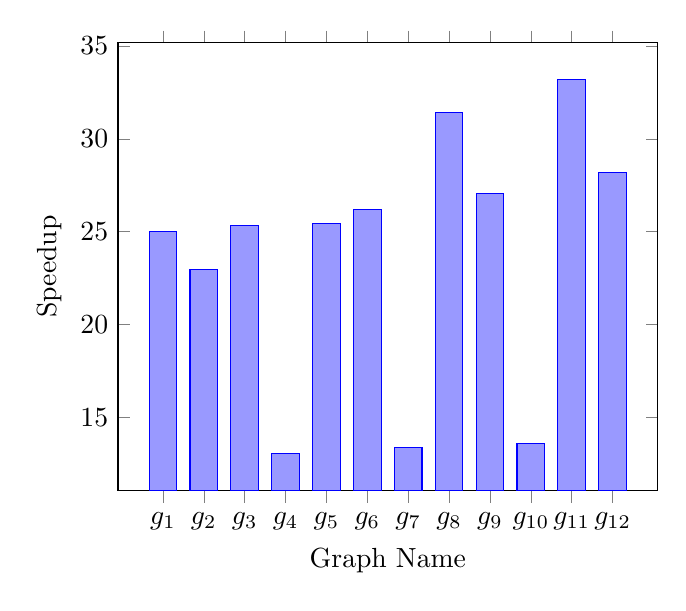
\begin{tikzpicture}
\begin{axis}[
    ybar,                   % Single series vertical bars chart
    ylabel={Speedup},
    xlabel={Graph Name},
    xtick=data,
    symbolic x coords={
        \(g_1\), \(g_2\), \(g_3\), \(g_4\), \(g_5\), \(g_6\), \(g_7\), \(g_8\), \(g_9\), \(g_{10}\), \(g_{11}\), \(g_{12}\) 
    },
]

\addplot[fill=blue!40, draw=blue] coordinates {
    (\(g_1\), 25.00) (\(g_2\), 22.96) (\(g_3\), 25.34) 
    (\(g_4\), 13.08) (\(g_5\), 25.46) (\(g_6\), 26.20)
    (\(g_7\), 13.40) (\(g_8\), 31.41) (\(g_9\), 27.08)
    (\(g_{10}\), 13.63) (\(g_{11}\), 33.17) (\(g_{12}\), 28.18)
};

\end{axis}
\end{tikzpicture}
\caption{Speedup between the fastest CPU and the GPU implementations on different graphs (the HE-based implementations)}
\label{fig:speedup}
\end{figure}